\paragraph{Question 1}

\begin{itemize}
\item[] a) Le programme linéaire en nombre entier présenté dans
  l'énoncé se justifie de la manière suivante~:
\begin{itemize}
\item $x_j \in \{0,1\}, j=1..n$ car on a le choix binaire entre prendre un
  sommet (donc le compter avec 1), ou ne pas le prendre (ne pas le
  compter avec 0, élement neutre de l'addition). Il y a bien
  évidemment n sommets, d'où l'indexation de 1 à n.
\item $min z = \sum^n _{i=1} x_i$ car on souhaite minimiser le nombre
  de sommets pris.
\item $x_r + x_s \geq 1$ car au moins un sommet doit être pris pour
  couvrir une arête.
\end{itemize}
Ces trois conditions décrivent donc bien le problème de la couverture minimale.
\item[] b) Le cas du triangle est un contre-exemple qui contredit cette
égalité. En effet (cf le dessin ci-dessous) le fait de
choisir l'arête $AC$, par exemple, empêcherait de sélectionner les
autres arêtes (sous peine de violer la contrainte d'égalité) alors
qu'un sommet resterait insaturé. Cette condition doit donc être
élargie à une inégalité.
\begin{figure}[!ht]
\begin{center}
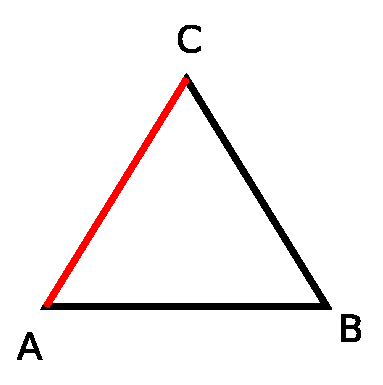
\includegraphics[height=3cm]{triangle.eps}
\end{center}
\caption{Pourquoi on ne peut pas avoir $x_r + x_S = 1$.}
\end{figure}
\item[] c) Montrons par l'absurde que le programme linéaire en nombres
  entiers est une borne inférieure de toute solution optimale.
\begin{proof}
Supposons que pour une instance donnée, on ait une solution optimale
de vertex cover qui soit meilleure que PLNE. Cela veut donc dire que
PLNE garde au au moins un sommet <<~en trop~>>. Or PLNE devrait
minimiser le nombre de sommets et le simplexe est adéquat. Le résultat
est donc absurde et contredit notre hypothèse de départ.
\end{proof}
\item[] d) Nous allons ici montrer de deux manières différentes que la
  relaxation des contraintes d'intégrité implique $x_r \geq
  \frac{1}{2}$ ou $x_s \geq \frac{1}{2}$.
\begin{itemize}
\item Première démonstration.
\begin{proof}
On veut, malgré la relaxation des contraintes d'intégrité, conserver
l'inégalité $x_r + x_s \geq 1$. Ainsi, on a $\neg (x_r + x_s < 1)$
d'où $\neg (x_r < \frac{1}{2} \wedge x_s < \frac{1}{2})$, et donc
($x_r \geq \frac{1}{2} \vee x_s \geq \frac{1}{2}) $ de par la loi de
De Morgan.
\end{proof}
\item Deuxième démonstration.
\begin{proof}
On sait que $A \Rightarrow B \equiv \neg A \vee B$. 
Or, pour respecter l'inégalité $x_r + x_s \geq 1$, on a $(x_r <
\frac{1}{2} \Rightarrow x_s \geq \frac{1}{2})$. On a ainsi $(x_r \geq
\frac{1}{2} \vee x_s \geq \frac{1}{2})$. 
\end{proof}
\end{itemize}
\item[] e) Montrons que l'algorithme 1 conduit à un algorithme
  approché avec une performance relative de de deux. 
\begin{proof}
Soit $C^{*}$ une solution optimale du problème de la couverture de
sommet. Soit $C$ la solution donnée par l'algorithme. 
$x_r=x_s=\frac{1}{2}$. Après la phase d'arrondi $x_r=x_s= 1$. D'où $
OPT = \frac{approche}{2}$.
En effet, on a pour exemple de pire des cas un carré, cf figure
ci-dessous.
\end{proof}

\begin{figure}
\begin{center}
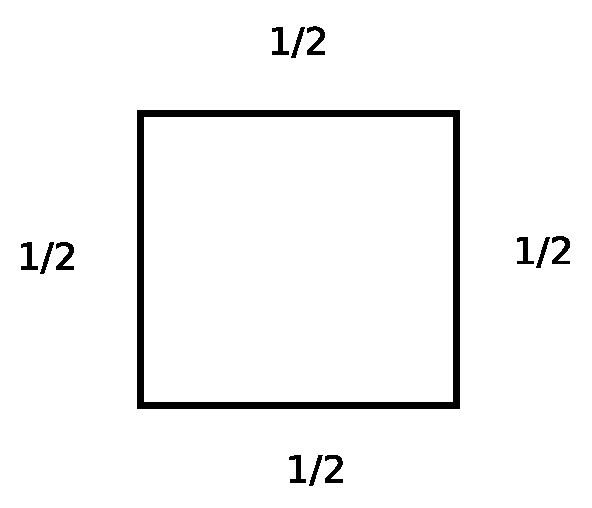
\includegraphics[height=3cm]{carre.eps}
\end{center}
\caption{Pire des cas pour l'algorithme 1}
\end{figure}

\item[] f)
\begin{itemize}
\item i)
Le programme linéaire correspondant à rajouter un poids aux arêtes au
problème du vertex cover est le suivant~:
\begin{equation}
\begin{cases}
min \sum_{i=1}^n w_{i, j}x_i \\
x_r + x_s \geq 1 \\
x_i \in \{ 0, 1 \} \\
\end{cases}
\end{equation}
\item ii)
\begin{equation}
\begin{cases}
min w^Tx \\
A^Tx \geq 1 \\
x_j \in \{0, 1\} \\
\end{cases}
\end{equation}
avec A matrice d'incidence sommets-arêtes.
\item iii) \begin{proof}
$x_i^*\geq \frac{1}{2} \Rightarrow x_i = 1$ \\
$x_i \leq 2x_i^*$ \\
$\Rightarrow C_{PLNE}=\sum x_iw_i \leq (2x_i^*)w_i \leq 2C_{opt}$ \\
\end{proof}
\end{itemize}
\end{itemize}

\paragraph{Question 2}

\begin{itemize}
\item[] a) Montrons que l'algorithme 2 est 2-approché.
\begin{proof}
Soit $C^{*}$ une solution optimale du problème de la couverture de
sommet. Soit $C$ la solution donnée par l'algorithme. 
\begin{itemize}
\item[] $|M| \leq C^{*}$ car deux arêtes adjacentes peuvent être
  couvertes par un même sommet.
\item[] $C^{*} \leq C = 2 |M|$ car une arête a deux sommets.
\item[] On a donc $\frac{C}{C^{*}} \leq \frac{2|M|}{|M|} = 2$.
\end{itemize}
\end{proof}
\item[] b) Il suffit de prendre $C_4$.
\item[] c) 
\begin{itemize}
\item[] Dans le pire des cas donné à la figure 1, l'algorithme renvoie
  une solution $C$ de taille 8. Or la solution optimale $C^*$ pour cette
  instance est de taille 5. En effet, aucun des sommets de plus haut
  degré n'est inclus dans $C^{*}$. Le choix du sommet de plus haut
  degré n'est donc pas une bonne heuristique. 
\item[] En revanche, on peut remarquer que cet algorithme trouve la
  solution optimale sur $C_4$ (qui était le cas limite de l'algorithme 2).
\end{itemize}
\end{itemize}
